% !TeX program = lualatex
% Standalone plot: Monomials x^2, x^3, x^4, x^5 on [-1,1]

\documentclass[tikz, border=5pt]{standalone}
\usepackage{pgfplots}
\pgfplotsset{compat=newest}
\begin{document}
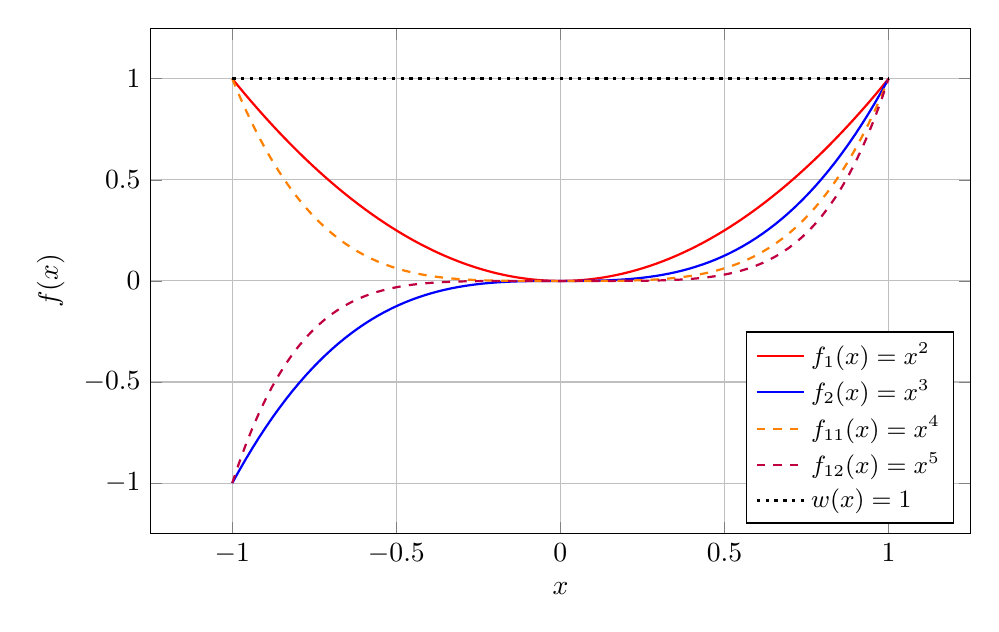
\begin{tikzpicture}
  \begin{axis}[
    width=12cm,
    height=8cm,
    xmin=-1.25, xmax=1.25,
    ymin=-1.25, ymax=1.25,
    xlabel={$x$}, ylabel={$f(x)$},
    xtick={-1,-0.5,0,0.5,1},
    ytick={-1,-0.5,0,0.5,1},
    grid=both,
    legend style={at={(0.98,0.02)},anchor=south east, font=\small},
    legend cell align={left},
    samples=100
  ]
    % x^2
    \addplot[domain=-1:1, thick, color=red] {x^2};
    \addlegendentry{$f_1(x) = x^2$}
    % x^3
    \addplot[domain=-1:1, thick, color=blue] {x^3};
    \addlegendentry{$f_2(x) = x^3$}
    % x^4
    \addplot[domain=-1:1, thick, color=orange, dashed] {x^4};
    \addlegendentry{$f_{11}(x) = x^4$}
    % x^5
    \addplot[domain=-1:1, thick, color=purple, dashed] {x^5};
    \addlegendentry{$f_{12}(x) = x^5$}
    % w(x) = 1 (horizontal line at y=1)
    \addplot[domain=-1:1, very thick, color=black, dotted] {1};
    \addlegendentry{$w(x) = 1$}
  \end{axis}
\end{tikzpicture}
\end{document}
